\documentclass[aspectratio=169]{beamer}
% Shared preamble for ml/ slide decks.
% Each lecture .tex starts with:
%   \documentclass[aspectratio=169]{beamer}
%   % Shared preamble for ml/ slide decks.
% Each lecture .tex starts with:
%   \documentclass[aspectratio=169]{beamer}
%   % Shared preamble for ml/ slide decks.
% Each lecture .tex starts with:
%   \documentclass[aspectratio=169]{beamer}
%   \input{../preamble}
% Compile from inside the chapter folder so \input{../preamble} resolves.

\usetheme{default}
\usecolortheme{dove}

\setbeamertemplate{navigation symbols}{}
\setbeamertemplate{footline}{%
  \hfill{\large\insertframenumber\,/\,\inserttotalframenumber}\hspace{0.8em}\vspace{0.5em}%
}

% Project palette (existing, kept for backwards compatibility with deferred/*)
\definecolor{popblue}{RGB}{52, 101, 164}
\definecolor{sampred}{RGB}{204, 0, 0}
\definecolor{paramgreen}{RGB}{0, 140, 70}
\definecolor{warnred}{RGB}{180, 40, 40}
\definecolor{orange1}{RGB}{220, 120, 0}
\definecolor{violet1}{RGB}{120, 50, 160}
\definecolor{lightbg}{RGB}{245, 245, 250}

% Armenian flag palette (use these for any 3-color highlight; per CLAUDE.md).
% "Nice versions": slightly de-saturated from the official spec for slide use,
% so they don't burn out under projector colors. Originals kept as *_pure.
\definecolor{armred}{RGB}{200, 30, 40}      % nice red (official #D90012 muted)
\definecolor{armblue}{RGB}{30, 70, 160}     % nice blue (official #0033A0 muted)
\definecolor{armorange}{RGB}{230, 160, 30}  % nice orange (official #F2A800 muted)
\definecolor{armred_pure}{HTML}{D90012}     % official Armenian flag red
\definecolor{armblue_pure}{HTML}{0033A0}    % official Armenian flag blue
\definecolor{armorange_pure}{HTML}{F2A800}  % official Armenian flag orange

\setbeamercolor{frametitle}{fg=popblue}
\setbeamercolor{title}{fg=popblue}

\usepackage{pgfplots}
\usepackage{tikz}
\usetikzlibrary{shapes, arrows.meta, positioning, calc, decorations.pathreplacing, patterns, matrix}
\pgfplotsset{compat=1.18}
\usepackage{amsmath, amssymb, amsfonts}
\usepackage{bm}
\usepackage{dsfont}
\usepackage{array}
\usepackage{pifont}
\usepackage{colortbl}
\usepackage{fontenc}

% Callout boxes. Purely additive - existing decks are unaffected.
% Usage: \begin{tcolorbox}[colback=armblue!8, colframe=armblue, boxrule=0.6pt, arc=2pt,
%                          title=\textbf{Key idea}] ... \end{tcolorbox}
% Palette convention (ml/SLIDE_STYLE.md): armblue=key idea, armred=trap/warning,
% paramgreen=takeaway or "Next", armorange=watch-out.
\usepackage[most]{tcolorbox}

% Cleaner table rules (\toprule, \midrule, \bottomrule). Also purely additive.
\usepackage{booktabs}

% \cancel{...} for struck-through terms in derivations (added 2026-08-11 for the
% importance-sampling frame in ch11_rl, where the dynamics cancel). Purely additive.
\usepackage{cancel}

% Minimal ML notation macros (subset of slds-lmu latex-math/basic-ml.tex).
% Kept here so we don't have to inline-expand every \thetav, \xv, etc.
% when porting upstream slides.
\newcommand{\R}{\mathds{R}}
\newcommand{\N}{\mathds{N}}
\newcommand{\E}{\mathds{E}}
\newcommand{\Xspace}{\mathcal{X}}
\newcommand{\Yspace}{\mathcal{Y}}
\newcommand{\Hspace}{\mathcal{H}}
\newcommand{\D}{\mathcal{D}}
\newcommand{\Dtrain}{\mathcal{D}_{\text{train}}}
\newcommand{\Dtest}{\mathcal{D}_{\text{test}}}
\newcommand{\xv}{\mathbf{x}}
\newcommand{\yv}{\mathbf{y}}
\newcommand{\Xmat}{\mathbf{X}}
\newcommand{\id}{\mathbf{I}}
\newcommand{\thetav}{\bm{\theta}}
\newcommand{\thetah}{\hat{\bm{\theta}}}
\newcommand{\lamv}{\bm{\lambda}}
\newcommand{\fx}{f(\xv)}
\newcommand{\fxt}{f(\xv \,|\, \bm{\theta})}
\newcommand{\fxi}{f\!\left(\xv^{(i)}\right)}
\newcommand{\fh}{\hat{f}}
\newcommand{\fxh}{\hat{f}(\xv)}
\newcommand{\yh}{\hat{y}}
\newcommand{\yih}{\hat{y}^{(i)}}
% \xi clashes with the Greek letter \xi; write \xv^{(i)} inline instead.
\newcommand{\yi}[1][i]{y^{(#1)}}
\newcommand{\xyi}[1][i]{\left(\xv^{(#1)},\, y^{(#1)}\right)}
\newcommand{\thx}{\bm{\theta}^\top \xv}
\newcommand{\sumin}{\sum_{i=1}^{n}}
\newcommand{\sumjp}{\sum_{j=1}^{p}}
\newcommand{\Lxy}{L\!\left(y, \fx\right)}
\newcommand{\Lxyi}{L\!\left(\yi, \fxi\right)}
\newcommand{\risk}{\mathcal{R}}
\newcommand{\riske}{\mathcal{R}_{\text{emp}}}
\newcommand{\risket}{\mathcal{R}_{\text{emp}}(\bm{\theta})}
\newcommand{\riskt}{\mathcal{R}(\bm{\theta})}
\newcommand{\riskr}{\mathcal{R}_{\text{reg}}}
\newcommand{\argmin}{\mathop{\mathrm{arg\,min}}}
\newcommand{\argmax}{\mathop{\mathrm{arg\,max}}}
\newcommand{\eps}{\varepsilon}

% Compile from inside the chapter folder so % Shared preamble for ml/ slide decks.
% Each lecture .tex starts with:
%   \documentclass[aspectratio=169]{beamer}
%   \input{../preamble}
% Compile from inside the chapter folder so \input{../preamble} resolves.

\usetheme{default}
\usecolortheme{dove}

\setbeamertemplate{navigation symbols}{}
\setbeamertemplate{footline}{%
  \hfill{\large\insertframenumber\,/\,\inserttotalframenumber}\hspace{0.8em}\vspace{0.5em}%
}

% Project palette (existing, kept for backwards compatibility with deferred/*)
\definecolor{popblue}{RGB}{52, 101, 164}
\definecolor{sampred}{RGB}{204, 0, 0}
\definecolor{paramgreen}{RGB}{0, 140, 70}
\definecolor{warnred}{RGB}{180, 40, 40}
\definecolor{orange1}{RGB}{220, 120, 0}
\definecolor{violet1}{RGB}{120, 50, 160}
\definecolor{lightbg}{RGB}{245, 245, 250}

% Armenian flag palette (use these for any 3-color highlight; per CLAUDE.md).
% "Nice versions": slightly de-saturated from the official spec for slide use,
% so they don't burn out under projector colors. Originals kept as *_pure.
\definecolor{armred}{RGB}{200, 30, 40}      % nice red (official #D90012 muted)
\definecolor{armblue}{RGB}{30, 70, 160}     % nice blue (official #0033A0 muted)
\definecolor{armorange}{RGB}{230, 160, 30}  % nice orange (official #F2A800 muted)
\definecolor{armred_pure}{HTML}{D90012}     % official Armenian flag red
\definecolor{armblue_pure}{HTML}{0033A0}    % official Armenian flag blue
\definecolor{armorange_pure}{HTML}{F2A800}  % official Armenian flag orange

\setbeamercolor{frametitle}{fg=popblue}
\setbeamercolor{title}{fg=popblue}

\usepackage{pgfplots}
\usepackage{tikz}
\usetikzlibrary{shapes, arrows.meta, positioning, calc, decorations.pathreplacing, patterns, matrix}
\pgfplotsset{compat=1.18}
\usepackage{amsmath, amssymb, amsfonts}
\usepackage{bm}
\usepackage{dsfont}
\usepackage{array}
\usepackage{pifont}
\usepackage{colortbl}
\usepackage{fontenc}

% Callout boxes. Purely additive - existing decks are unaffected.
% Usage: \begin{tcolorbox}[colback=armblue!8, colframe=armblue, boxrule=0.6pt, arc=2pt,
%                          title=\textbf{Key idea}] ... \end{tcolorbox}
% Palette convention (ml/SLIDE_STYLE.md): armblue=key idea, armred=trap/warning,
% paramgreen=takeaway or "Next", armorange=watch-out.
\usepackage[most]{tcolorbox}

% Cleaner table rules (\toprule, \midrule, \bottomrule). Also purely additive.
\usepackage{booktabs}

% \cancel{...} for struck-through terms in derivations (added 2026-08-11 for the
% importance-sampling frame in ch11_rl, where the dynamics cancel). Purely additive.
\usepackage{cancel}

% Minimal ML notation macros (subset of slds-lmu latex-math/basic-ml.tex).
% Kept here so we don't have to inline-expand every \thetav, \xv, etc.
% when porting upstream slides.
\newcommand{\R}{\mathds{R}}
\newcommand{\N}{\mathds{N}}
\newcommand{\E}{\mathds{E}}
\newcommand{\Xspace}{\mathcal{X}}
\newcommand{\Yspace}{\mathcal{Y}}
\newcommand{\Hspace}{\mathcal{H}}
\newcommand{\D}{\mathcal{D}}
\newcommand{\Dtrain}{\mathcal{D}_{\text{train}}}
\newcommand{\Dtest}{\mathcal{D}_{\text{test}}}
\newcommand{\xv}{\mathbf{x}}
\newcommand{\yv}{\mathbf{y}}
\newcommand{\Xmat}{\mathbf{X}}
\newcommand{\id}{\mathbf{I}}
\newcommand{\thetav}{\bm{\theta}}
\newcommand{\thetah}{\hat{\bm{\theta}}}
\newcommand{\lamv}{\bm{\lambda}}
\newcommand{\fx}{f(\xv)}
\newcommand{\fxt}{f(\xv \,|\, \bm{\theta})}
\newcommand{\fxi}{f\!\left(\xv^{(i)}\right)}
\newcommand{\fh}{\hat{f}}
\newcommand{\fxh}{\hat{f}(\xv)}
\newcommand{\yh}{\hat{y}}
\newcommand{\yih}{\hat{y}^{(i)}}
% \xi clashes with the Greek letter \xi; write \xv^{(i)} inline instead.
\newcommand{\yi}[1][i]{y^{(#1)}}
\newcommand{\xyi}[1][i]{\left(\xv^{(#1)},\, y^{(#1)}\right)}
\newcommand{\thx}{\bm{\theta}^\top \xv}
\newcommand{\sumin}{\sum_{i=1}^{n}}
\newcommand{\sumjp}{\sum_{j=1}^{p}}
\newcommand{\Lxy}{L\!\left(y, \fx\right)}
\newcommand{\Lxyi}{L\!\left(\yi, \fxi\right)}
\newcommand{\risk}{\mathcal{R}}
\newcommand{\riske}{\mathcal{R}_{\text{emp}}}
\newcommand{\risket}{\mathcal{R}_{\text{emp}}(\bm{\theta})}
\newcommand{\riskt}{\mathcal{R}(\bm{\theta})}
\newcommand{\riskr}{\mathcal{R}_{\text{reg}}}
\newcommand{\argmin}{\mathop{\mathrm{arg\,min}}}
\newcommand{\argmax}{\mathop{\mathrm{arg\,max}}}
\newcommand{\eps}{\varepsilon}
 resolves.

\usetheme{default}
\usecolortheme{dove}

\setbeamertemplate{navigation symbols}{}
\setbeamertemplate{footline}{%
  \hfill{\large\insertframenumber\,/\,\inserttotalframenumber}\hspace{0.8em}\vspace{0.5em}%
}

% Project palette (existing, kept for backwards compatibility with deferred/*)
\definecolor{popblue}{RGB}{52, 101, 164}
\definecolor{sampred}{RGB}{204, 0, 0}
\definecolor{paramgreen}{RGB}{0, 140, 70}
\definecolor{warnred}{RGB}{180, 40, 40}
\definecolor{orange1}{RGB}{220, 120, 0}
\definecolor{violet1}{RGB}{120, 50, 160}
\definecolor{lightbg}{RGB}{245, 245, 250}

% Armenian flag palette (use these for any 3-color highlight; per CLAUDE.md).
% "Nice versions": slightly de-saturated from the official spec for slide use,
% so they don't burn out under projector colors. Originals kept as *_pure.
\definecolor{armred}{RGB}{200, 30, 40}      % nice red (official #D90012 muted)
\definecolor{armblue}{RGB}{30, 70, 160}     % nice blue (official #0033A0 muted)
\definecolor{armorange}{RGB}{230, 160, 30}  % nice orange (official #F2A800 muted)
\definecolor{armred_pure}{HTML}{D90012}     % official Armenian flag red
\definecolor{armblue_pure}{HTML}{0033A0}    % official Armenian flag blue
\definecolor{armorange_pure}{HTML}{F2A800}  % official Armenian flag orange

\setbeamercolor{frametitle}{fg=popblue}
\setbeamercolor{title}{fg=popblue}

\usepackage{pgfplots}
\usepackage{tikz}
\usetikzlibrary{shapes, arrows.meta, positioning, calc, decorations.pathreplacing, patterns, matrix}
\pgfplotsset{compat=1.18}
\usepackage{amsmath, amssymb, amsfonts}
\usepackage{bm}
\usepackage{dsfont}
\usepackage{array}
\usepackage{pifont}
\usepackage{colortbl}
\usepackage{fontenc}

% Callout boxes. Purely additive - existing decks are unaffected.
% Usage: \begin{tcolorbox}[colback=armblue!8, colframe=armblue, boxrule=0.6pt, arc=2pt,
%                          title=\textbf{Key idea}] ... \end{tcolorbox}
% Palette convention (ml/SLIDE_STYLE.md): armblue=key idea, armred=trap/warning,
% paramgreen=takeaway or "Next", armorange=watch-out.
\usepackage[most]{tcolorbox}

% Cleaner table rules (\toprule, \midrule, \bottomrule). Also purely additive.
\usepackage{booktabs}

% \cancel{...} for struck-through terms in derivations (added 2026-08-11 for the
% importance-sampling frame in ch11_rl, where the dynamics cancel). Purely additive.
\usepackage{cancel}

% Minimal ML notation macros (subset of slds-lmu latex-math/basic-ml.tex).
% Kept here so we don't have to inline-expand every \thetav, \xv, etc.
% when porting upstream slides.
\newcommand{\R}{\mathds{R}}
\newcommand{\N}{\mathds{N}}
\newcommand{\E}{\mathds{E}}
\newcommand{\Xspace}{\mathcal{X}}
\newcommand{\Yspace}{\mathcal{Y}}
\newcommand{\Hspace}{\mathcal{H}}
\newcommand{\D}{\mathcal{D}}
\newcommand{\Dtrain}{\mathcal{D}_{\text{train}}}
\newcommand{\Dtest}{\mathcal{D}_{\text{test}}}
\newcommand{\xv}{\mathbf{x}}
\newcommand{\yv}{\mathbf{y}}
\newcommand{\Xmat}{\mathbf{X}}
\newcommand{\id}{\mathbf{I}}
\newcommand{\thetav}{\bm{\theta}}
\newcommand{\thetah}{\hat{\bm{\theta}}}
\newcommand{\lamv}{\bm{\lambda}}
\newcommand{\fx}{f(\xv)}
\newcommand{\fxt}{f(\xv \,|\, \bm{\theta})}
\newcommand{\fxi}{f\!\left(\xv^{(i)}\right)}
\newcommand{\fh}{\hat{f}}
\newcommand{\fxh}{\hat{f}(\xv)}
\newcommand{\yh}{\hat{y}}
\newcommand{\yih}{\hat{y}^{(i)}}
% \xi clashes with the Greek letter \xi; write \xv^{(i)} inline instead.
\newcommand{\yi}[1][i]{y^{(#1)}}
\newcommand{\xyi}[1][i]{\left(\xv^{(#1)},\, y^{(#1)}\right)}
\newcommand{\thx}{\bm{\theta}^\top \xv}
\newcommand{\sumin}{\sum_{i=1}^{n}}
\newcommand{\sumjp}{\sum_{j=1}^{p}}
\newcommand{\Lxy}{L\!\left(y, \fx\right)}
\newcommand{\Lxyi}{L\!\left(\yi, \fxi\right)}
\newcommand{\risk}{\mathcal{R}}
\newcommand{\riske}{\mathcal{R}_{\text{emp}}}
\newcommand{\risket}{\mathcal{R}_{\text{emp}}(\bm{\theta})}
\newcommand{\riskt}{\mathcal{R}(\bm{\theta})}
\newcommand{\riskr}{\mathcal{R}_{\text{reg}}}
\newcommand{\argmin}{\mathop{\mathrm{arg\,min}}}
\newcommand{\argmax}{\mathop{\mathrm{arg\,max}}}
\newcommand{\eps}{\varepsilon}

% Compile from inside the chapter folder so % Shared preamble for ml/ slide decks.
% Each lecture .tex starts with:
%   \documentclass[aspectratio=169]{beamer}
%   % Shared preamble for ml/ slide decks.
% Each lecture .tex starts with:
%   \documentclass[aspectratio=169]{beamer}
%   \input{../preamble}
% Compile from inside the chapter folder so \input{../preamble} resolves.

\usetheme{default}
\usecolortheme{dove}

\setbeamertemplate{navigation symbols}{}
\setbeamertemplate{footline}{%
  \hfill{\large\insertframenumber\,/\,\inserttotalframenumber}\hspace{0.8em}\vspace{0.5em}%
}

% Project palette (existing, kept for backwards compatibility with deferred/*)
\definecolor{popblue}{RGB}{52, 101, 164}
\definecolor{sampred}{RGB}{204, 0, 0}
\definecolor{paramgreen}{RGB}{0, 140, 70}
\definecolor{warnred}{RGB}{180, 40, 40}
\definecolor{orange1}{RGB}{220, 120, 0}
\definecolor{violet1}{RGB}{120, 50, 160}
\definecolor{lightbg}{RGB}{245, 245, 250}

% Armenian flag palette (use these for any 3-color highlight; per CLAUDE.md).
% "Nice versions": slightly de-saturated from the official spec for slide use,
% so they don't burn out under projector colors. Originals kept as *_pure.
\definecolor{armred}{RGB}{200, 30, 40}      % nice red (official #D90012 muted)
\definecolor{armblue}{RGB}{30, 70, 160}     % nice blue (official #0033A0 muted)
\definecolor{armorange}{RGB}{230, 160, 30}  % nice orange (official #F2A800 muted)
\definecolor{armred_pure}{HTML}{D90012}     % official Armenian flag red
\definecolor{armblue_pure}{HTML}{0033A0}    % official Armenian flag blue
\definecolor{armorange_pure}{HTML}{F2A800}  % official Armenian flag orange

\setbeamercolor{frametitle}{fg=popblue}
\setbeamercolor{title}{fg=popblue}

\usepackage{pgfplots}
\usepackage{tikz}
\usetikzlibrary{shapes, arrows.meta, positioning, calc, decorations.pathreplacing, patterns, matrix}
\pgfplotsset{compat=1.18}
\usepackage{amsmath, amssymb, amsfonts}
\usepackage{bm}
\usepackage{dsfont}
\usepackage{array}
\usepackage{pifont}
\usepackage{colortbl}
\usepackage{fontenc}

% Callout boxes. Purely additive - existing decks are unaffected.
% Usage: \begin{tcolorbox}[colback=armblue!8, colframe=armblue, boxrule=0.6pt, arc=2pt,
%                          title=\textbf{Key idea}] ... \end{tcolorbox}
% Palette convention (ml/SLIDE_STYLE.md): armblue=key idea, armred=trap/warning,
% paramgreen=takeaway or "Next", armorange=watch-out.
\usepackage[most]{tcolorbox}

% Cleaner table rules (\toprule, \midrule, \bottomrule). Also purely additive.
\usepackage{booktabs}

% \cancel{...} for struck-through terms in derivations (added 2026-08-11 for the
% importance-sampling frame in ch11_rl, where the dynamics cancel). Purely additive.
\usepackage{cancel}

% Minimal ML notation macros (subset of slds-lmu latex-math/basic-ml.tex).
% Kept here so we don't have to inline-expand every \thetav, \xv, etc.
% when porting upstream slides.
\newcommand{\R}{\mathds{R}}
\newcommand{\N}{\mathds{N}}
\newcommand{\E}{\mathds{E}}
\newcommand{\Xspace}{\mathcal{X}}
\newcommand{\Yspace}{\mathcal{Y}}
\newcommand{\Hspace}{\mathcal{H}}
\newcommand{\D}{\mathcal{D}}
\newcommand{\Dtrain}{\mathcal{D}_{\text{train}}}
\newcommand{\Dtest}{\mathcal{D}_{\text{test}}}
\newcommand{\xv}{\mathbf{x}}
\newcommand{\yv}{\mathbf{y}}
\newcommand{\Xmat}{\mathbf{X}}
\newcommand{\id}{\mathbf{I}}
\newcommand{\thetav}{\bm{\theta}}
\newcommand{\thetah}{\hat{\bm{\theta}}}
\newcommand{\lamv}{\bm{\lambda}}
\newcommand{\fx}{f(\xv)}
\newcommand{\fxt}{f(\xv \,|\, \bm{\theta})}
\newcommand{\fxi}{f\!\left(\xv^{(i)}\right)}
\newcommand{\fh}{\hat{f}}
\newcommand{\fxh}{\hat{f}(\xv)}
\newcommand{\yh}{\hat{y}}
\newcommand{\yih}{\hat{y}^{(i)}}
% \xi clashes with the Greek letter \xi; write \xv^{(i)} inline instead.
\newcommand{\yi}[1][i]{y^{(#1)}}
\newcommand{\xyi}[1][i]{\left(\xv^{(#1)},\, y^{(#1)}\right)}
\newcommand{\thx}{\bm{\theta}^\top \xv}
\newcommand{\sumin}{\sum_{i=1}^{n}}
\newcommand{\sumjp}{\sum_{j=1}^{p}}
\newcommand{\Lxy}{L\!\left(y, \fx\right)}
\newcommand{\Lxyi}{L\!\left(\yi, \fxi\right)}
\newcommand{\risk}{\mathcal{R}}
\newcommand{\riske}{\mathcal{R}_{\text{emp}}}
\newcommand{\risket}{\mathcal{R}_{\text{emp}}(\bm{\theta})}
\newcommand{\riskt}{\mathcal{R}(\bm{\theta})}
\newcommand{\riskr}{\mathcal{R}_{\text{reg}}}
\newcommand{\argmin}{\mathop{\mathrm{arg\,min}}}
\newcommand{\argmax}{\mathop{\mathrm{arg\,max}}}
\newcommand{\eps}{\varepsilon}

% Compile from inside the chapter folder so % Shared preamble for ml/ slide decks.
% Each lecture .tex starts with:
%   \documentclass[aspectratio=169]{beamer}
%   \input{../preamble}
% Compile from inside the chapter folder so \input{../preamble} resolves.

\usetheme{default}
\usecolortheme{dove}

\setbeamertemplate{navigation symbols}{}
\setbeamertemplate{footline}{%
  \hfill{\large\insertframenumber\,/\,\inserttotalframenumber}\hspace{0.8em}\vspace{0.5em}%
}

% Project palette (existing, kept for backwards compatibility with deferred/*)
\definecolor{popblue}{RGB}{52, 101, 164}
\definecolor{sampred}{RGB}{204, 0, 0}
\definecolor{paramgreen}{RGB}{0, 140, 70}
\definecolor{warnred}{RGB}{180, 40, 40}
\definecolor{orange1}{RGB}{220, 120, 0}
\definecolor{violet1}{RGB}{120, 50, 160}
\definecolor{lightbg}{RGB}{245, 245, 250}

% Armenian flag palette (use these for any 3-color highlight; per CLAUDE.md).
% "Nice versions": slightly de-saturated from the official spec for slide use,
% so they don't burn out under projector colors. Originals kept as *_pure.
\definecolor{armred}{RGB}{200, 30, 40}      % nice red (official #D90012 muted)
\definecolor{armblue}{RGB}{30, 70, 160}     % nice blue (official #0033A0 muted)
\definecolor{armorange}{RGB}{230, 160, 30}  % nice orange (official #F2A800 muted)
\definecolor{armred_pure}{HTML}{D90012}     % official Armenian flag red
\definecolor{armblue_pure}{HTML}{0033A0}    % official Armenian flag blue
\definecolor{armorange_pure}{HTML}{F2A800}  % official Armenian flag orange

\setbeamercolor{frametitle}{fg=popblue}
\setbeamercolor{title}{fg=popblue}

\usepackage{pgfplots}
\usepackage{tikz}
\usetikzlibrary{shapes, arrows.meta, positioning, calc, decorations.pathreplacing, patterns, matrix}
\pgfplotsset{compat=1.18}
\usepackage{amsmath, amssymb, amsfonts}
\usepackage{bm}
\usepackage{dsfont}
\usepackage{array}
\usepackage{pifont}
\usepackage{colortbl}
\usepackage{fontenc}

% Callout boxes. Purely additive - existing decks are unaffected.
% Usage: \begin{tcolorbox}[colback=armblue!8, colframe=armblue, boxrule=0.6pt, arc=2pt,
%                          title=\textbf{Key idea}] ... \end{tcolorbox}
% Palette convention (ml/SLIDE_STYLE.md): armblue=key idea, armred=trap/warning,
% paramgreen=takeaway or "Next", armorange=watch-out.
\usepackage[most]{tcolorbox}

% Cleaner table rules (\toprule, \midrule, \bottomrule). Also purely additive.
\usepackage{booktabs}

% \cancel{...} for struck-through terms in derivations (added 2026-08-11 for the
% importance-sampling frame in ch11_rl, where the dynamics cancel). Purely additive.
\usepackage{cancel}

% Minimal ML notation macros (subset of slds-lmu latex-math/basic-ml.tex).
% Kept here so we don't have to inline-expand every \thetav, \xv, etc.
% when porting upstream slides.
\newcommand{\R}{\mathds{R}}
\newcommand{\N}{\mathds{N}}
\newcommand{\E}{\mathds{E}}
\newcommand{\Xspace}{\mathcal{X}}
\newcommand{\Yspace}{\mathcal{Y}}
\newcommand{\Hspace}{\mathcal{H}}
\newcommand{\D}{\mathcal{D}}
\newcommand{\Dtrain}{\mathcal{D}_{\text{train}}}
\newcommand{\Dtest}{\mathcal{D}_{\text{test}}}
\newcommand{\xv}{\mathbf{x}}
\newcommand{\yv}{\mathbf{y}}
\newcommand{\Xmat}{\mathbf{X}}
\newcommand{\id}{\mathbf{I}}
\newcommand{\thetav}{\bm{\theta}}
\newcommand{\thetah}{\hat{\bm{\theta}}}
\newcommand{\lamv}{\bm{\lambda}}
\newcommand{\fx}{f(\xv)}
\newcommand{\fxt}{f(\xv \,|\, \bm{\theta})}
\newcommand{\fxi}{f\!\left(\xv^{(i)}\right)}
\newcommand{\fh}{\hat{f}}
\newcommand{\fxh}{\hat{f}(\xv)}
\newcommand{\yh}{\hat{y}}
\newcommand{\yih}{\hat{y}^{(i)}}
% \xi clashes with the Greek letter \xi; write \xv^{(i)} inline instead.
\newcommand{\yi}[1][i]{y^{(#1)}}
\newcommand{\xyi}[1][i]{\left(\xv^{(#1)},\, y^{(#1)}\right)}
\newcommand{\thx}{\bm{\theta}^\top \xv}
\newcommand{\sumin}{\sum_{i=1}^{n}}
\newcommand{\sumjp}{\sum_{j=1}^{p}}
\newcommand{\Lxy}{L\!\left(y, \fx\right)}
\newcommand{\Lxyi}{L\!\left(\yi, \fxi\right)}
\newcommand{\risk}{\mathcal{R}}
\newcommand{\riske}{\mathcal{R}_{\text{emp}}}
\newcommand{\risket}{\mathcal{R}_{\text{emp}}(\bm{\theta})}
\newcommand{\riskt}{\mathcal{R}(\bm{\theta})}
\newcommand{\riskr}{\mathcal{R}_{\text{reg}}}
\newcommand{\argmin}{\mathop{\mathrm{arg\,min}}}
\newcommand{\argmax}{\mathop{\mathrm{arg\,max}}}
\newcommand{\eps}{\varepsilon}
 resolves.

\usetheme{default}
\usecolortheme{dove}

\setbeamertemplate{navigation symbols}{}
\setbeamertemplate{footline}{%
  \hfill{\large\insertframenumber\,/\,\inserttotalframenumber}\hspace{0.8em}\vspace{0.5em}%
}

% Project palette (existing, kept for backwards compatibility with deferred/*)
\definecolor{popblue}{RGB}{52, 101, 164}
\definecolor{sampred}{RGB}{204, 0, 0}
\definecolor{paramgreen}{RGB}{0, 140, 70}
\definecolor{warnred}{RGB}{180, 40, 40}
\definecolor{orange1}{RGB}{220, 120, 0}
\definecolor{violet1}{RGB}{120, 50, 160}
\definecolor{lightbg}{RGB}{245, 245, 250}

% Armenian flag palette (use these for any 3-color highlight; per CLAUDE.md).
% "Nice versions": slightly de-saturated from the official spec for slide use,
% so they don't burn out under projector colors. Originals kept as *_pure.
\definecolor{armred}{RGB}{200, 30, 40}      % nice red (official #D90012 muted)
\definecolor{armblue}{RGB}{30, 70, 160}     % nice blue (official #0033A0 muted)
\definecolor{armorange}{RGB}{230, 160, 30}  % nice orange (official #F2A800 muted)
\definecolor{armred_pure}{HTML}{D90012}     % official Armenian flag red
\definecolor{armblue_pure}{HTML}{0033A0}    % official Armenian flag blue
\definecolor{armorange_pure}{HTML}{F2A800}  % official Armenian flag orange

\setbeamercolor{frametitle}{fg=popblue}
\setbeamercolor{title}{fg=popblue}

\usepackage{pgfplots}
\usepackage{tikz}
\usetikzlibrary{shapes, arrows.meta, positioning, calc, decorations.pathreplacing, patterns, matrix}
\pgfplotsset{compat=1.18}
\usepackage{amsmath, amssymb, amsfonts}
\usepackage{bm}
\usepackage{dsfont}
\usepackage{array}
\usepackage{pifont}
\usepackage{colortbl}
\usepackage{fontenc}

% Callout boxes. Purely additive - existing decks are unaffected.
% Usage: \begin{tcolorbox}[colback=armblue!8, colframe=armblue, boxrule=0.6pt, arc=2pt,
%                          title=\textbf{Key idea}] ... \end{tcolorbox}
% Palette convention (ml/SLIDE_STYLE.md): armblue=key idea, armred=trap/warning,
% paramgreen=takeaway or "Next", armorange=watch-out.
\usepackage[most]{tcolorbox}

% Cleaner table rules (\toprule, \midrule, \bottomrule). Also purely additive.
\usepackage{booktabs}

% \cancel{...} for struck-through terms in derivations (added 2026-08-11 for the
% importance-sampling frame in ch11_rl, where the dynamics cancel). Purely additive.
\usepackage{cancel}

% Minimal ML notation macros (subset of slds-lmu latex-math/basic-ml.tex).
% Kept here so we don't have to inline-expand every \thetav, \xv, etc.
% when porting upstream slides.
\newcommand{\R}{\mathds{R}}
\newcommand{\N}{\mathds{N}}
\newcommand{\E}{\mathds{E}}
\newcommand{\Xspace}{\mathcal{X}}
\newcommand{\Yspace}{\mathcal{Y}}
\newcommand{\Hspace}{\mathcal{H}}
\newcommand{\D}{\mathcal{D}}
\newcommand{\Dtrain}{\mathcal{D}_{\text{train}}}
\newcommand{\Dtest}{\mathcal{D}_{\text{test}}}
\newcommand{\xv}{\mathbf{x}}
\newcommand{\yv}{\mathbf{y}}
\newcommand{\Xmat}{\mathbf{X}}
\newcommand{\id}{\mathbf{I}}
\newcommand{\thetav}{\bm{\theta}}
\newcommand{\thetah}{\hat{\bm{\theta}}}
\newcommand{\lamv}{\bm{\lambda}}
\newcommand{\fx}{f(\xv)}
\newcommand{\fxt}{f(\xv \,|\, \bm{\theta})}
\newcommand{\fxi}{f\!\left(\xv^{(i)}\right)}
\newcommand{\fh}{\hat{f}}
\newcommand{\fxh}{\hat{f}(\xv)}
\newcommand{\yh}{\hat{y}}
\newcommand{\yih}{\hat{y}^{(i)}}
% \xi clashes with the Greek letter \xi; write \xv^{(i)} inline instead.
\newcommand{\yi}[1][i]{y^{(#1)}}
\newcommand{\xyi}[1][i]{\left(\xv^{(#1)},\, y^{(#1)}\right)}
\newcommand{\thx}{\bm{\theta}^\top \xv}
\newcommand{\sumin}{\sum_{i=1}^{n}}
\newcommand{\sumjp}{\sum_{j=1}^{p}}
\newcommand{\Lxy}{L\!\left(y, \fx\right)}
\newcommand{\Lxyi}{L\!\left(\yi, \fxi\right)}
\newcommand{\risk}{\mathcal{R}}
\newcommand{\riske}{\mathcal{R}_{\text{emp}}}
\newcommand{\risket}{\mathcal{R}_{\text{emp}}(\bm{\theta})}
\newcommand{\riskt}{\mathcal{R}(\bm{\theta})}
\newcommand{\riskr}{\mathcal{R}_{\text{reg}}}
\newcommand{\argmin}{\mathop{\mathrm{arg\,min}}}
\newcommand{\argmax}{\mathop{\mathrm{arg\,max}}}
\newcommand{\eps}{\varepsilon}
 resolves.

\usetheme{default}
\usecolortheme{dove}

\setbeamertemplate{navigation symbols}{}
\setbeamertemplate{footline}{%
  \hfill{\large\insertframenumber\,/\,\inserttotalframenumber}\hspace{0.8em}\vspace{0.5em}%
}

% Project palette (existing, kept for backwards compatibility with deferred/*)
\definecolor{popblue}{RGB}{52, 101, 164}
\definecolor{sampred}{RGB}{204, 0, 0}
\definecolor{paramgreen}{RGB}{0, 140, 70}
\definecolor{warnred}{RGB}{180, 40, 40}
\definecolor{orange1}{RGB}{220, 120, 0}
\definecolor{violet1}{RGB}{120, 50, 160}
\definecolor{lightbg}{RGB}{245, 245, 250}

% Armenian flag palette (use these for any 3-color highlight; per CLAUDE.md).
% "Nice versions": slightly de-saturated from the official spec for slide use,
% so they don't burn out under projector colors. Originals kept as *_pure.
\definecolor{armred}{RGB}{200, 30, 40}      % nice red (official #D90012 muted)
\definecolor{armblue}{RGB}{30, 70, 160}     % nice blue (official #0033A0 muted)
\definecolor{armorange}{RGB}{230, 160, 30}  % nice orange (official #F2A800 muted)
\definecolor{armred_pure}{HTML}{D90012}     % official Armenian flag red
\definecolor{armblue_pure}{HTML}{0033A0}    % official Armenian flag blue
\definecolor{armorange_pure}{HTML}{F2A800}  % official Armenian flag orange

\setbeamercolor{frametitle}{fg=popblue}
\setbeamercolor{title}{fg=popblue}

\usepackage{pgfplots}
\usepackage{tikz}
\usetikzlibrary{shapes, arrows.meta, positioning, calc, decorations.pathreplacing, patterns, matrix}
\pgfplotsset{compat=1.18}
\usepackage{amsmath, amssymb, amsfonts}
\usepackage{bm}
\usepackage{dsfont}
\usepackage{array}
\usepackage{pifont}
\usepackage{colortbl}
\usepackage{fontenc}

% Callout boxes. Purely additive - existing decks are unaffected.
% Usage: \begin{tcolorbox}[colback=armblue!8, colframe=armblue, boxrule=0.6pt, arc=2pt,
%                          title=\textbf{Key idea}] ... \end{tcolorbox}
% Palette convention (ml/SLIDE_STYLE.md): armblue=key idea, armred=trap/warning,
% paramgreen=takeaway or "Next", armorange=watch-out.
\usepackage[most]{tcolorbox}

% Cleaner table rules (\toprule, \midrule, \bottomrule). Also purely additive.
\usepackage{booktabs}

% \cancel{...} for struck-through terms in derivations (added 2026-08-11 for the
% importance-sampling frame in ch11_rl, where the dynamics cancel). Purely additive.
\usepackage{cancel}

% Minimal ML notation macros (subset of slds-lmu latex-math/basic-ml.tex).
% Kept here so we don't have to inline-expand every \thetav, \xv, etc.
% when porting upstream slides.
\newcommand{\R}{\mathds{R}}
\newcommand{\N}{\mathds{N}}
\newcommand{\E}{\mathds{E}}
\newcommand{\Xspace}{\mathcal{X}}
\newcommand{\Yspace}{\mathcal{Y}}
\newcommand{\Hspace}{\mathcal{H}}
\newcommand{\D}{\mathcal{D}}
\newcommand{\Dtrain}{\mathcal{D}_{\text{train}}}
\newcommand{\Dtest}{\mathcal{D}_{\text{test}}}
\newcommand{\xv}{\mathbf{x}}
\newcommand{\yv}{\mathbf{y}}
\newcommand{\Xmat}{\mathbf{X}}
\newcommand{\id}{\mathbf{I}}
\newcommand{\thetav}{\bm{\theta}}
\newcommand{\thetah}{\hat{\bm{\theta}}}
\newcommand{\lamv}{\bm{\lambda}}
\newcommand{\fx}{f(\xv)}
\newcommand{\fxt}{f(\xv \,|\, \bm{\theta})}
\newcommand{\fxi}{f\!\left(\xv^{(i)}\right)}
\newcommand{\fh}{\hat{f}}
\newcommand{\fxh}{\hat{f}(\xv)}
\newcommand{\yh}{\hat{y}}
\newcommand{\yih}{\hat{y}^{(i)}}
% \xi clashes with the Greek letter \xi; write \xv^{(i)} inline instead.
\newcommand{\yi}[1][i]{y^{(#1)}}
\newcommand{\xyi}[1][i]{\left(\xv^{(#1)},\, y^{(#1)}\right)}
\newcommand{\thx}{\bm{\theta}^\top \xv}
\newcommand{\sumin}{\sum_{i=1}^{n}}
\newcommand{\sumjp}{\sum_{j=1}^{p}}
\newcommand{\Lxy}{L\!\left(y, \fx\right)}
\newcommand{\Lxyi}{L\!\left(\yi, \fxi\right)}
\newcommand{\risk}{\mathcal{R}}
\newcommand{\riske}{\mathcal{R}_{\text{emp}}}
\newcommand{\risket}{\mathcal{R}_{\text{emp}}(\bm{\theta})}
\newcommand{\riskt}{\mathcal{R}(\bm{\theta})}
\newcommand{\riskr}{\mathcal{R}_{\text{reg}}}
\newcommand{\argmin}{\mathop{\mathrm{arg\,min}}}
\newcommand{\argmax}{\mathop{\mathrm{arg\,max}}}
\newcommand{\eps}{\varepsilon}


\graphicspath{{fig/}}

% callout boxes, matching the chapter's fcolorbox house pattern (LLM-1 to LLM-11)
\newcommand{\keybox}[1]{\fcolorbox{armblue}{armblue!8}{\parbox{0.97\linewidth}{\small #1}}}
\newcommand{\trapbox}[1]{\fcolorbox{armred}{armred!8}{\parbox{0.97\linewidth}{\small #1}}}
\newcommand{\takebox}[1]{\fcolorbox{paramgreen}{paramgreen!8}{\parbox{0.97\linewidth}{\small #1}}}
\newcommand{\watchbox}[1]{\fcolorbox{armorange}{armorange!12}{\parbox{0.97\linewidth}{\small #1}}}

\newcommand{\sectiontransition}[2]{%
  \begin{frame}[plain]
    \vfill
    \begin{center}
      {\Huge\bfseries\color{popblue} #1}\\[1.1em]
      {\large #2}
    \end{center}
    \vfill
  \end{frame}}

\newcommand{\src}[1]{{\scriptsize\color{gray} #1}}

\title{Quantization}
\subtitle{An LLM on your laptop}
\author{}
\date{}

\begin{document}

\begin{frame}[plain]
  \titlepage
  \begin{center}\scriptsize\color{gray}
    LLM chapter, session 12. Toy numbers unless a slide says otherwise.
  \end{center}
\end{frame}

% ============================================================ WHERE WE ARE (py_src/llm_roadmap.py)
\begin{frame}{Where we are: one forward pass}
  \begin{center}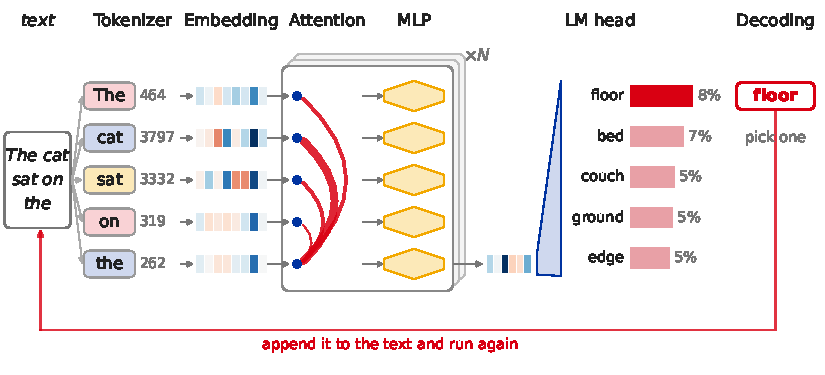
\includegraphics[width=\linewidth]{roadmap_quantization_pass.pdf}\end{center}
  \vskip -2pt
  {\small Every box of the pass multiplies by stored weights. Today: store them in fewer bits.}
\end{frame}

\begin{frame}{Where we are: the life of a model}
  \begin{center}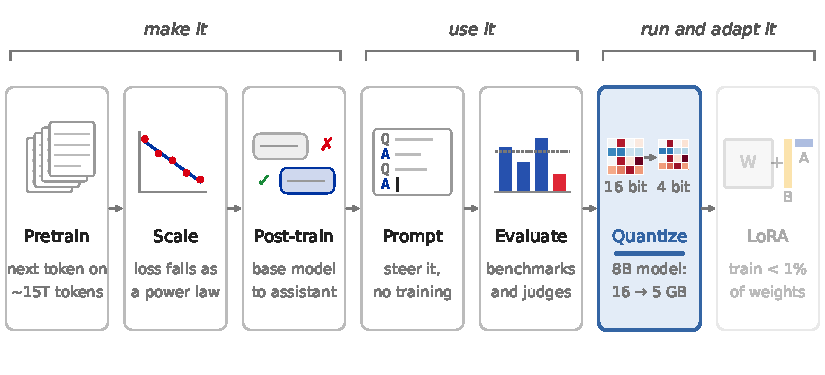
\includegraphics[width=\linewidth]{roadmap_quantization_life.pdf}\end{center}
  \vskip -2pt
  {\small Today: the first box of ``run and adapt it''.}
\end{frame}

% ============================================================ COLD OPEN (py_src/quant_figs.py --gpt2)
\begin{frame}{Does it fit?}
  \vskip 8pt
  \begin{itemize}
    \item An 8B model in bf16: $8 \times 10^9 \times 2$ bytes $= 16$ GB.
    \item This laptop: 16 GB of memory - for everything, the operating system included.
    \item At 4 bits per weight it would be about 4 GB (4.5 GB with the scales; real 4-bit files
      keep a few tensors at higher precision, so the map rounds to 5).
  \end{itemize}

  \vskip 14pt
  \trapbox{\textbf{Predict first:} store every weight in 4 bits instead of 16 or 32. How much
  worse does the model get - a little, or completely?}
\end{frame}

\begin{frame}{GPT-2 at 4 bits, two ways}
  \begin{center}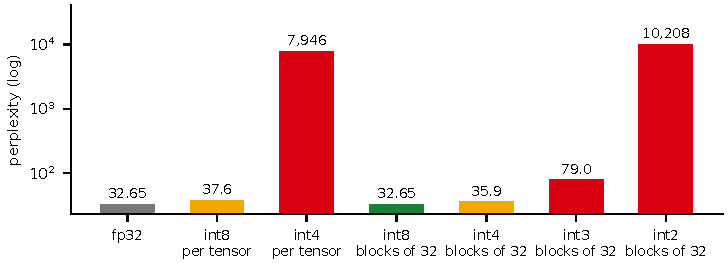
\includegraphics[width=0.84\linewidth]{quant_ladder.pdf}\end{center}
  \vskip -4pt
  {\small Real: GPT-2's 48 block weight matrices rounded in NumPy, perplexity measured with the cached
  model on 8,192 tokens of wikitext (LLM-7's perplexity; lower is better). One scale per matrix at 4
  bits: 7,946 - destroyed. A scale per block of 32 weights: 35.9, against 32.65 in fp32.}

  \vskip 4pt
  \keybox{\textbf{Answer: both.} Same 4 bits, opposite results; even 8 bits with one scale (37.6)
  loses to 4 bits in blocks. A \textbf{scale} maps the stored integers back to real numbers, and
  where it comes from matters more than the bit count - this lecture's main idea.}
\end{frame}

\begin{frame}{Outline}
  \tableofcontents
\end{frame}

% ============================================================ 1. THE BILL
\section{The bill}
\sectiontransition{The bill}{Every weight and every cached token costs bytes.}

\begin{frame}{Memory, by hand}
  \vskip 6pt
  \textbf{Weights}: parameters $\times$ bytes per parameter.
  \vskip 4pt
  \begin{center}
  \begin{tabular}{lrr}
    \toprule
    & \textbf{GPT-2 small} & \textbf{an 8B model} \\
    \midrule
    parameters & 124,439,808 & $8 \times 10^9$ \\
    fp32, 4 bytes & 498 MB & 32 GB \\
    bf16, 2 bytes & 249 MB & 16 GB \\
    4.5 bits (4-bit blocks) & 70 MB & 4.5 GB \\
    \bottomrule
  \end{tabular}
  \end{center}

  \vskip 8pt
  \keybox{Training needed about 16 bytes per parameter (LLM-8). Running needs only the weights -
  and they can shrink further.}
\end{frame}

\begin{frame}{The KV cache}
  \begin{columns}[c]
    \column{0.60\textwidth}
      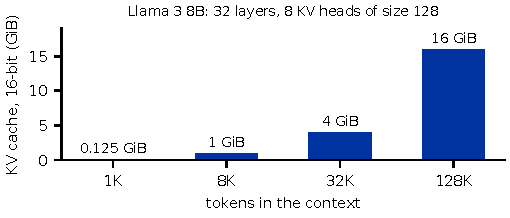
\includegraphics[width=\linewidth]{quant_kv.pdf}
    \column{0.38\textwidth}
      {\small Generating, the model keeps every earlier token's keys and values (LLM-3) so it does
      not recompute them. Per token:
      \vskip 3pt
      $2 \times \text{layers} \times \text{KV heads} \times \text{head size} \times \text{bytes}$
      \vskip 2pt
      (the 2: one key and one value).}
  \end{columns}

  \vskip 6pt
  {\small \textbf{By hand}, 16-bit: GPT-2, $2 \times 12 \times 768 \times 2 = 36{,}864$ bytes per token,
  37.7 MB for 1,024 tokens. Llama 3 8B, $2 \times 32 \times 8 \times 128 \times 2 = 131{,}072$
  bytes (128 KiB): 1 GiB at 8K tokens, 16 GiB at 128K.}

  \vskip 4pt
  \watchbox{Long context costs memory too - at 128K about the size of the whole 16-bit model.
  Llama 3 keeps 8 key/value heads, not 32: 4$\times$ less. How that works: LLM-14.}
\end{frame}

\begin{frame}{Fewer bytes is also faster}
  \vskip 6pt
  \begin{itemize}
    \item Generating one token reads every weight once (one user; a dense model, where every
      weight is used for every token). The arithmetic is quick; moving the bytes is the slow part.
    \item So: tokens per second $\leq$ memory bandwidth (bytes per second the memory delivers)
      / bytes read per token.
    \item \textbf{Measured} on this laptop: a NumPy copy moves 15.7 GB/s, counting bytes read and
      written - an estimate. An 8B model at 16 GB (it would not even fit): at most 1.0 tokens/s.
      At 4.5 GB: at most 3.5 tokens/s. (The KV cache adds a little to each read.)
  \end{itemize}

  \vskip 10pt
  \takebox{Quantizing to 4 bits does not just make the model fit; it makes it up to about
  3.5$\times$ faster to generate on the same machine.}
\end{frame}

% ============================================================ 2. FEWER BITS
\section{Fewer bits}
\sectiontransition{Fewer bits}{What a number costs, and what rounding costs.}

\begin{frame}{Number formats}
  \begin{center}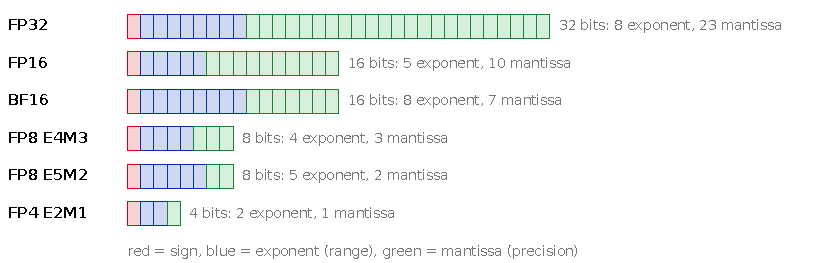
\includegraphics[width=\linewidth]{quant_formats.pdf}\end{center}
  \vskip -4pt
  \begin{itemize}
    \small
    \item A float stores a sign, an exponent (how big: the range) and a mantissa (how precise).
      BF16 keeps FP32's 8 exponent bits and drops precision; FP16 keeps more precision and loses
      range.
    \item Integers (INT8, INT4) have no exponent: one shared \textbf{scale} says how big the
      integers are. Everything today is about choosing that scale.
  \end{itemize}
\end{frame}

\begin{frame}{Absmax, by hand}
  \vskip 2pt
  Four weights: $[0.5, -1.1, 0.3, 2.4]$. Pick the scale so the largest becomes the largest integer:
  \vskip 4pt
  \begin{center}
  \small
  \begin{tabular}{lccc}
    \toprule
    & \textbf{scale} & \textbf{integers} & \textbf{back to numbers} \\
    \midrule
    INT8 (to $\pm 127$) & $2.4 / 127 = 0.0189$ & $[26, -58, 16, 127]$ & $[0.49, -1.10, 0.30, 2.40]$ \\
    INT4 (to $\pm 7$) & $2.4 / 7 = 0.343$ & $[1, -3, 1, 7]$ & $[0.34, -1.03, 0.34, 2.40]$ \\
    \bottomrule
  \end{tabular}
  \end{center}
  \vskip 6pt
  {\small integer $= \text{round}(w / \text{scale})$; \quad back $=$ integer $\times$ scale. Store the
  integers and one scale.}

  \vskip 6pt
  \keybox{At 4 bits there are only 15 levels ($-7$ to $7$), so every weight moves to its nearest
  level: $0.5 \to 0.34$. The largest weight sets the step size for all of them.}
\end{frame}

\begin{frame}{One outlier}
  \begin{center}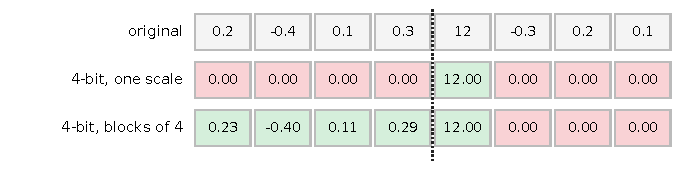
\includegraphics[width=0.84\linewidth]{quant_outlier.pdf}\end{center}
  \vskip -4pt
  {\small Toy numbers. One weight is 12.0, the others below 0.5. With one scale for all eight, the
  step is $12/7 = 1.7$, so every small weight rounds to 0 (red; green = kept). With a scale per
  block of 4 (dotted line), only the block that holds the outlier suffers.}

  \vskip 4pt
  \keybox{That is the cold open: a few large \emph{weights} in each GPT-2 matrix, and one scale per
  matrix zeroes out most of the rest. Blocks keep the damage local.}
\end{frame}

\begin{frame}{Blocks, and their price}
  \vskip 6pt
  \begin{itemize}
    \item Each block stores its own scale, usually 16 bits. Bits per weight:
      \quad $4 + 16/32 = $ \textbf{4.5} for 4-bit blocks of 32.
    \item GPT-2, blocks of 32: 8 bits - no loss (32.65 both); 4 bits - 35.9; 3 bits - 79.0; 2
      bits - 10,208.
    \item Hardware formats bake this in. \textbf{MXFP4} (an open standard): blocks of 32 4-bit
      floats with an 8-bit power-of-two scale. \textbf{NVFP4} (NVIDIA): blocks of 16 with an FP8
      scale, plus one scale for the whole tensor.
  \end{itemize}

  \vskip 8pt
  \takebox{Smaller blocks fit the local numbers better and cost more scale bits. Around 4 bits per
  weight is where most local models run today.}
\end{frame}

\begin{frame}{Outliers in real models}
  \vskip 6pt
  \begin{itemize}
    \item A second kind of outlier, in the \emph{activations} (the values flowing between layers,
      not the stored weights): in large models a few dimensions are huge. Dettmers et al. (2022): handle those dimensions in 16 bits and ``more than
      99.9\% of values'' can still be multiplied in 8 bits (LLM.int8()).
    \item Activations change with every input; weights are fixed and can be studied once.
    \item So the common path on laptops: quantize the \textbf{weights} only, keep the activations
      in 16 bits. Each 4-bit weight is turned back into 16 bits (integer $\times$ scale) just before
      it is used; it is stored in 4.
  \end{itemize}

  \vskip 10pt
  \watchbox{Weight-only quantization saves memory and bandwidth - the two things that limit a
  laptop. The arithmetic still happens in 16 bits.}
\end{frame}

% ============================================================ 3. SMARTER THAN ROUNDING
\section{Smarter than rounding}
\sectiontransition{Smarter than rounding}{Fix the errors rounding makes.}

\begin{frame}{Correct the error}
  \vskip 6pt
  \begin{itemize}
    \item Rounding treats each weight alone. But a layer's output is a sum: if one weight rounds
      down, others can be nudged to make up for it.
    \item \textbf{GPTQ} (Frantar et al., 2022): quantize a layer one column at a time, and after
      each step adjust the not-yet-quantized weights to cancel the error, using a small sample of
      real inputs (a calibration set).
    \item \textbf{AWQ} (Lin et al., 2023): find the input channels that carry large activations
      and protect their weights by scaling them up before rounding.
  \end{itemize}

  \vskip 10pt
  \keybox{Both quantize a finished model (PTQ, ``post-training quantization'' - not LLM-9's
  post-training): no retraining, minutes to hours. The details are optional; the idea is ``round,
  then repair''.}
\end{frame}

\begin{frame}{Train for it}
  \vskip 6pt
  \begin{itemize}
    \item \textbf{Quantization-aware training} (QAT): during training, round the weights in the
      forward pass, so the model learns to live with the rounding.
    \item gpt-oss (OpenAI, 2025) was trained with its expert weights in MXFP4. It is a mixture of
      experts: 21B parameters stored, only 3.6B used per token. It runs ``within 16GB of memory''.
    \item At the extreme: BitNet b1.58 trains ternary weights - only $-1$, $0$ or $+1$, $\log_2 3
      = 1.58$ bits each - from scratch.
  \end{itemize}

  \vskip 10pt
  \takebox{The best 4-bit model is one that was trained to be 4-bit. Rounding after the fact
  is the cheaper, more common path.}
\end{frame}

% ============================================================ 4. RUNNING IT
\section{Running it}
\sectiontransition{Running it}{The program between the file and your question.}

\begin{frame}{On this laptop, by hand}
  \vskip 6pt
  An 8B model at 4.5 bits per weight, on 16 GB:
  \vskip 4pt
  \begin{center}
  \begin{tabular}{lr}
    \toprule
    weights, $8 \times 10^9 \times 4.5 / 8$ bytes & 4.5 GB \\
    KV cache, 8K tokens of context (16-bit) & 1 GiB \\
    operating system, browser, the app & a few GB \\
    \midrule
    total & fits, with room \\
    \bottomrule
  \end{tabular}
  \end{center}
  \vskip 6pt
  {\small Speed: at most $15.7 / 4.5 \approx 3.5$ tokens per second from the measured bandwidth -
  readable, if not fast. In bf16 the same model would not load at all.}

  \vskip 6pt
  \takebox{That is the whole lecture in one table: fewer bits made it fit and made it faster.}
\end{frame}

\begin{frame}{What an inference engine does}
  \vskip 4pt
  A quantized file is just numbers. An \textbf{inference engine} is the program that turns it into
  answers. It exists because each of these is hard to do well:
  \vskip 4pt
  \begin{itemize}
    \item load the weights in their packed format, and multiply with them directly;
    \item keep and reuse the KV cache, and drop old entries when memory runs out;
    \item decode (LLM-6) and stream tokens as they come;
    \item serve many users at once by running their requests together (batching);
    \item offer an API that applications already know.
  \end{itemize}

  \vskip 6pt
  {\small Laptop engines optimise for one user on a CPU or a small GPU; server engines for many
  users on big GPUs. Names, as of October 2026: llama.cpp, Ollama and LM Studio on laptops; vLLM and
  SGLang on servers.}
\end{frame}

% ============================================================ CLOSE
\begin{frame}{Recap}
  \small
  \begin{itemize}
    \item \textbf{The bill}: weights cost parameters $\times$ bytes; the KV cache costs bytes per
      token and grows with the context. Generation is limited by memory bandwidth, so fewer bytes
      is also faster.
    \item \textbf{Fewer bits}: store integers and a scale. One scale per matrix lets one outlier
      ruin it (GPT-2 at 4 bits: 7,946); a scale per block of 32 keeps it (35.9).
    \item \textbf{Smarter than rounding}: correct the error (GPTQ, AWQ) or train for it (QAT,
      gpt-oss in MXFP4, ternary BitNet).
    \item \textbf{Running it}: an inference engine loads the packed weights, manages the cache and
      serves the answers.
  \end{itemize}
\end{frame}

\begin{frame}{Next on the map}
  \begin{center}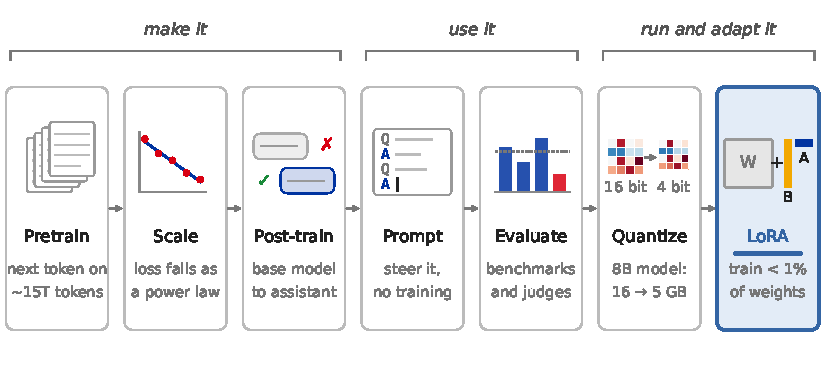
\includegraphics[width=\linewidth]{roadmap_lora_life.pdf}\end{center}
  \vskip -2pt
  {\small Next (LLM-13): adapting a model on a budget - LoRA, and QLoRA on a 4-bit base.}
\end{frame}

\begin{frame}{Sources \& further reading}
  \footnotesize
  \begin{itemize}
    \item Dettmers et al. (2022), ``LLM.int8(): 8-bit Matrix Multiplication for Transformers at
      Scale''.
    \item Frantar et al. (2022), ``GPTQ''; Lin et al. (2023), ``AWQ: Activation-aware Weight
      Quantization''.
    \item Open Compute Project, ``Microscaling Formats (MX) Specification''; NVIDIA, NVFP4.
    \item OpenAI (2025), gpt-oss model card; Ma et al. (2024), ``The Era of 1-bit LLMs'' (BitNet
      b1.58).
    \item Llama Team (2024), ``The Llama 3 Herd of Models'' (the 8B configuration).
  \end{itemize}
  \vskip 2pt
  \src{Figures: \texttt{py\_src/quant\_figs.py}. Real: GPT-2's perplexity at each precision
  (cached model, cached wikitext-2), this laptop's copy bandwidth. By hand: the memory and KV
  numbers. Toy: the absmax and outlier examples.}
\end{frame}

\end{document}

% ============================================================================
% Provenance:
%   Deck: LLM-12 Quantization (14_llms), session 12. Built 2026-10-06 from
%   LLM12_quantization_OUTLINE.md, which follows the critique in LLM_CHAPTER_PLAN.md (LLM-12) and
%   the queue (instructor: "do all queue items"): D4 answered - inference engines explained in
%   general, no runtime taught (DECISIONS #74); the measured ladder is GPT-2's own weights
%   quantized in NumPy (queue option (a), no downloads); homework skipped (no recommendation).
%   Sources ported: dl4nlp 11 (memory arithmetic, the quantization frames); llm_training 12
%   (blocks), 19 (float anatomy), 17 (FP8). The local-stack table and GGUF quant names were cut
%   (perishable; #74).
%   Facts checked 2026-10-06 (outline table): Llama 3 8B's configuration, MXFP4 / NVFP4, gpt-oss's
%   model card, LLM.int8()'s abstract.
%   Every printed number is asserted in py_src/quant_figs.py (the ladder, the memory and KV
%   numbers, the absmax table, the outlier toy, the bandwidth bound).
%   Found on the way: the KV chart drew 0 GiB at 32K / 128K - NumPy 1.26's int32 default on Windows
%   overflowed (_learnings/2026-10-06-2147_numpy-int32-default-on-windows-overflows-silently.md);
%   the plotted values are now checked too.
%   STUDENT REVIEW 2026-10-06 (one Sonnet agent, rendered PNGs only; ~79k tokens, 77 s). No
%   arithmetic errors. Applied: the answer to the predict and why int8 per tensor loses to int4 in
%   blocks; "scale" glossed at first use; weight outliers vs activation outliers told apart; the KV
%   chart Llama-only and the 2 explained; the bandwidth bound marked as an estimate and the 16 GB
%   case as hypothetical; PTQ vs LLM-9's post-training; MoE, QAT, ternary defined; dequantize
%   before the multiply; a new "On this laptop, by hand" frame (the title's promise).
% ============================================================================
